\section{Case Study 2: A simple OO modelling language}

This section presents a metamodel of a simple OO modelling language, which we call OML. OML is essentially a cut down version of UML and MOF. Whilst metamodels already exists for UML and MOF, they are complex, due to the rich set of modelling concepts they provide. Therefore, the metamodel presented here focuses on the most basic primitives necessary to express OO models.

As an example, figure \ref{omlexample} shows a simple model written in the language of OML.
The details of the model, a simple Bank in this case, are not particularly important. What is important is that it provides an example of the modelling concepts that are used by OML. These include the following:

\begin{figure}[htb]
\begin{center}
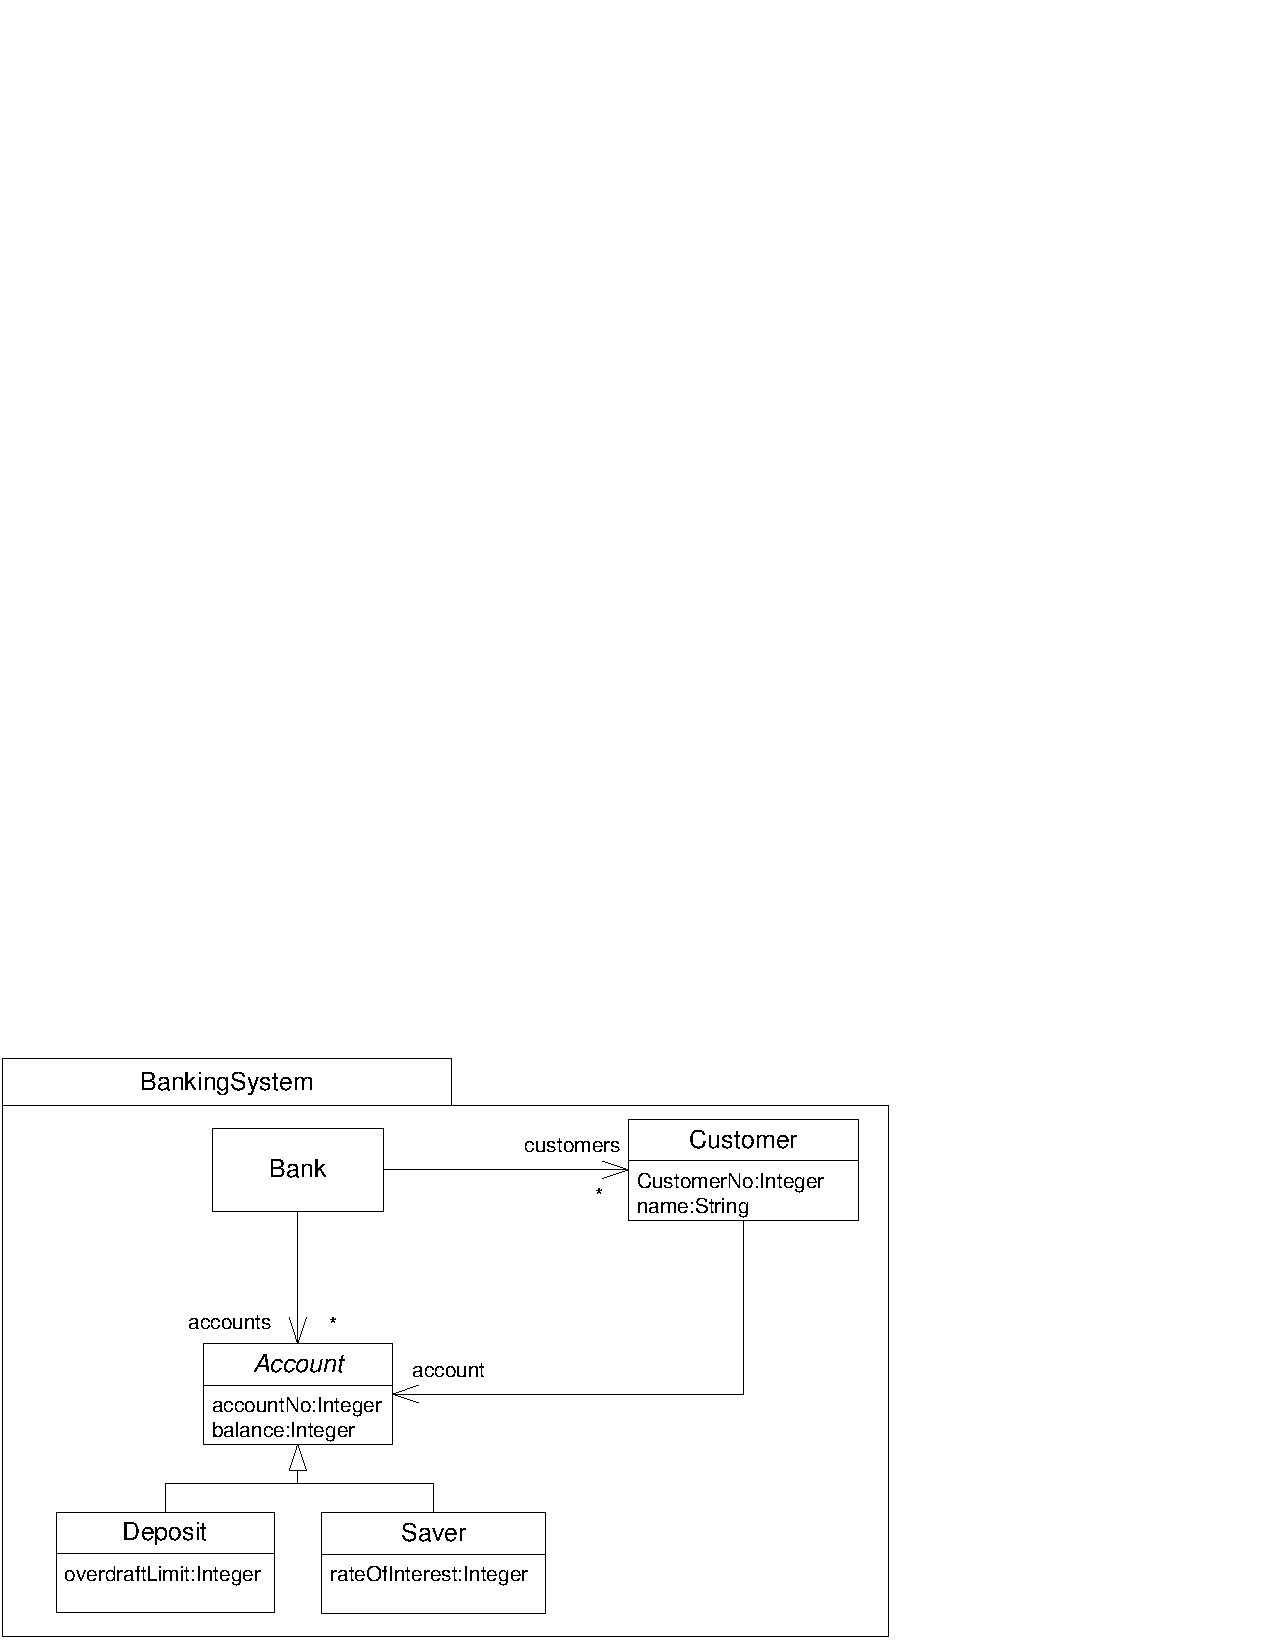
\includegraphics[width=13cm]{MetamodellingLanguages/StaticStructure/figures/OMLexample.pdf}
\caption{A simple OML model}
\label{omlexample}
\end{center}
\end{figure}

\begin{description}
\item [Class] A class is an abstraction of a collection of objects. A class has a name, and a set of attributes. A class may be related to another class by generalisation, in which case the more specific class is viewed as inheriting the properties of the more general class.
\item [Package] A package is a container of modelling elements, including classes. A package may contain other packages.
\item [Attribute] An attribute describes a particular property of a class. Attributes have a name and a type. A type may be a simple type, e.g. an Integer or a String, or a complex type, such as a class, or a collection of classes.
\end{description}

As explained in section, a useful exercise when identifying concepts in a language, is to annotate example models with the modelling concepts that they can be viewed as being instances of. Figure \ref{omlannotatedexample} shows the Bank example annotated with the modelling concepts that are in OML.

\begin{figure}[htb]
\begin{center}
\includegraphics[width=13cm]{MetamodellingLanguages/StaticStructure/figures/OMLannotatedexample.pdf}
\caption{An annotated OML model}
\label{omlannotatedexample}
\end{center}
\end{figure}

The representation of an attribute with a simple type versus an attribute with complex type is worth noting here. Whilst the concept is the same, the representation (concrete syntax) is quite different: a textual representation versus a diagrammatical one. In fact, there is nothing to prevent there being two or more ways of representing exactly the same concept. A textual representation of an attribute with a complex type could also have been used, e.g. accounts : Set{Account}.
As will be discussed in chapter{concretesyntax}, a concrete syntax merely provides (possibly multiple) views on the concepts in an abstract syntax metamodel.

\subsection{Metamodel}

Figure ? shows the result of translating the identified concepts into an abstractsyntax metamodel.